\documentclass{bioinfo}
\copyrightyear{2014}
\pubyear{2014}

\usepackage{hyperref}

\begin{document}
\firstpage{1}

%\title[short Title]{Structure prediction of globular proteins using predicted residue contacts.}
%\title[short Title]{PconsFold: ab-initio protein folding using Rosetta and predicted residue contacts.}
\title[PconsFold]{PconsFold: Protein folding using predicted residue contacts}
%\title[short Title]{Advancement in residue contact prediction improves quality of predicted structural models.}
%\author[Sample \textit{et~al}]{Mirco Michel\,$^{1,2}$, Marcin J. Skwark\,$^{3}$ and Arne Elofsson\,$^{1,2}$\footnote{to whom correspondence should be addressed}}
\author[M.Michel \textit{et~al}]{Mirco Michel\,$^{1,2}$, Sikander Hayat, Marcin Skwark, Debora Marks, and Arne Elofsson\,$^{1,2}$\footnote{to whom correspondence should be addressed}}
\address{$^{1}$Department of Biochemistry and Biophysics, Stockholm University, 10691 Stockholm, Sweden\\
$^{2}$Science for Life Laboratory, Box 1031, 17121 Solna, Sweden}
%$^{3}$Department of Information and Computer Science, Helsinki University of Technology TKK, Box 5400, FI-02015 TKK, Finland}

\history{Received on XXXXX; revised on XXXXX; accepted on XXXXX}

\editor{Associate Editor: XXXXXXX}

\maketitle

\begin{abstract}

\section{Motivation:}

\section{Results:}
Here we show that improved quality of evolutionary constraints increases quality and native-likeliness of predicted models. We also show that 
\section{Availability:}
We provide a fully automated pipeline, PconsFold, for predicting protein structures based on evolutionary information. PconsFold is based on PconsC and Rosetta and freely available at \url{https://www.github.com/ElofssonLab/pcons-fold}.
\section{Contact:} \href{arne@bioinfo.se}{arne@bioinfo.se}
\end{abstract}

\section{Introduction}
Predicting protein structures from sequences is one of the longest standing problems in structural biology. Although the problem itself remains unsolved, there has been continous effort and progress resulting in increased accuracy of predicted models \cite{casp}. 
Here we show that improved quality of evolutionary constraints increases quality and native-likeliness of predicted models. We elucidate diverging folding performance over different fold-classes. 
Structure prediction ab-initio still hard / motivate using sequence information to help structure prediction / residue contact map prediction improved dramatically / large amount of available sequences allows to use global models (DCA) instead of local models (MI) / now predicted contacts are precise enough to fascilitate ab-initio structure prediction / But what is the best way to do that? \\ 
Here we introduce a Rosetta folding protocol that uses residue contacts and includes these into the energy function / We benchmark our method on different datasets (PSICOV, Marks et al. 2013) / We compare our method to EVfold / 

Predicted contacts are used to constrain folding space / included in energy functions of Rosetta \& CNS \& Fragfold(?) / Benchmarked on different datasets(PSICOV, Marks et al. 2013, CASP10) / by calculating TM-scores of the top ranked models to the native structures / we investigate how many predicted contacts are needed for each method to attain highest accuracy / we optimize our Rosetta protocol in terms of runtime and accuracy / 

\begin{methods}
\section{Methods}
\subsection{Datasets}
\cite[]{jones_PSICOV:_2012}
\subsection{Residue-residue contact prediction}
For each protein $n = f \cdot l$ top ranked contacts were selected, where $l$ represents the length of the protein sequence and $f$ a factor to scale $n$ relative to the length.
\subsection{Rosetta}
We also used two different types of Rosetta energy functions, FADE and BOUNDED, for predicted contacts. Both functions are applied to all residue pairs that are assumed to be in spatial contact. Rosetta then calculates convert predicted contacts into distance based energies. 
\subsection{Model quality assessment}

\begin{figure}[!tpb]%figure1
    \centerline{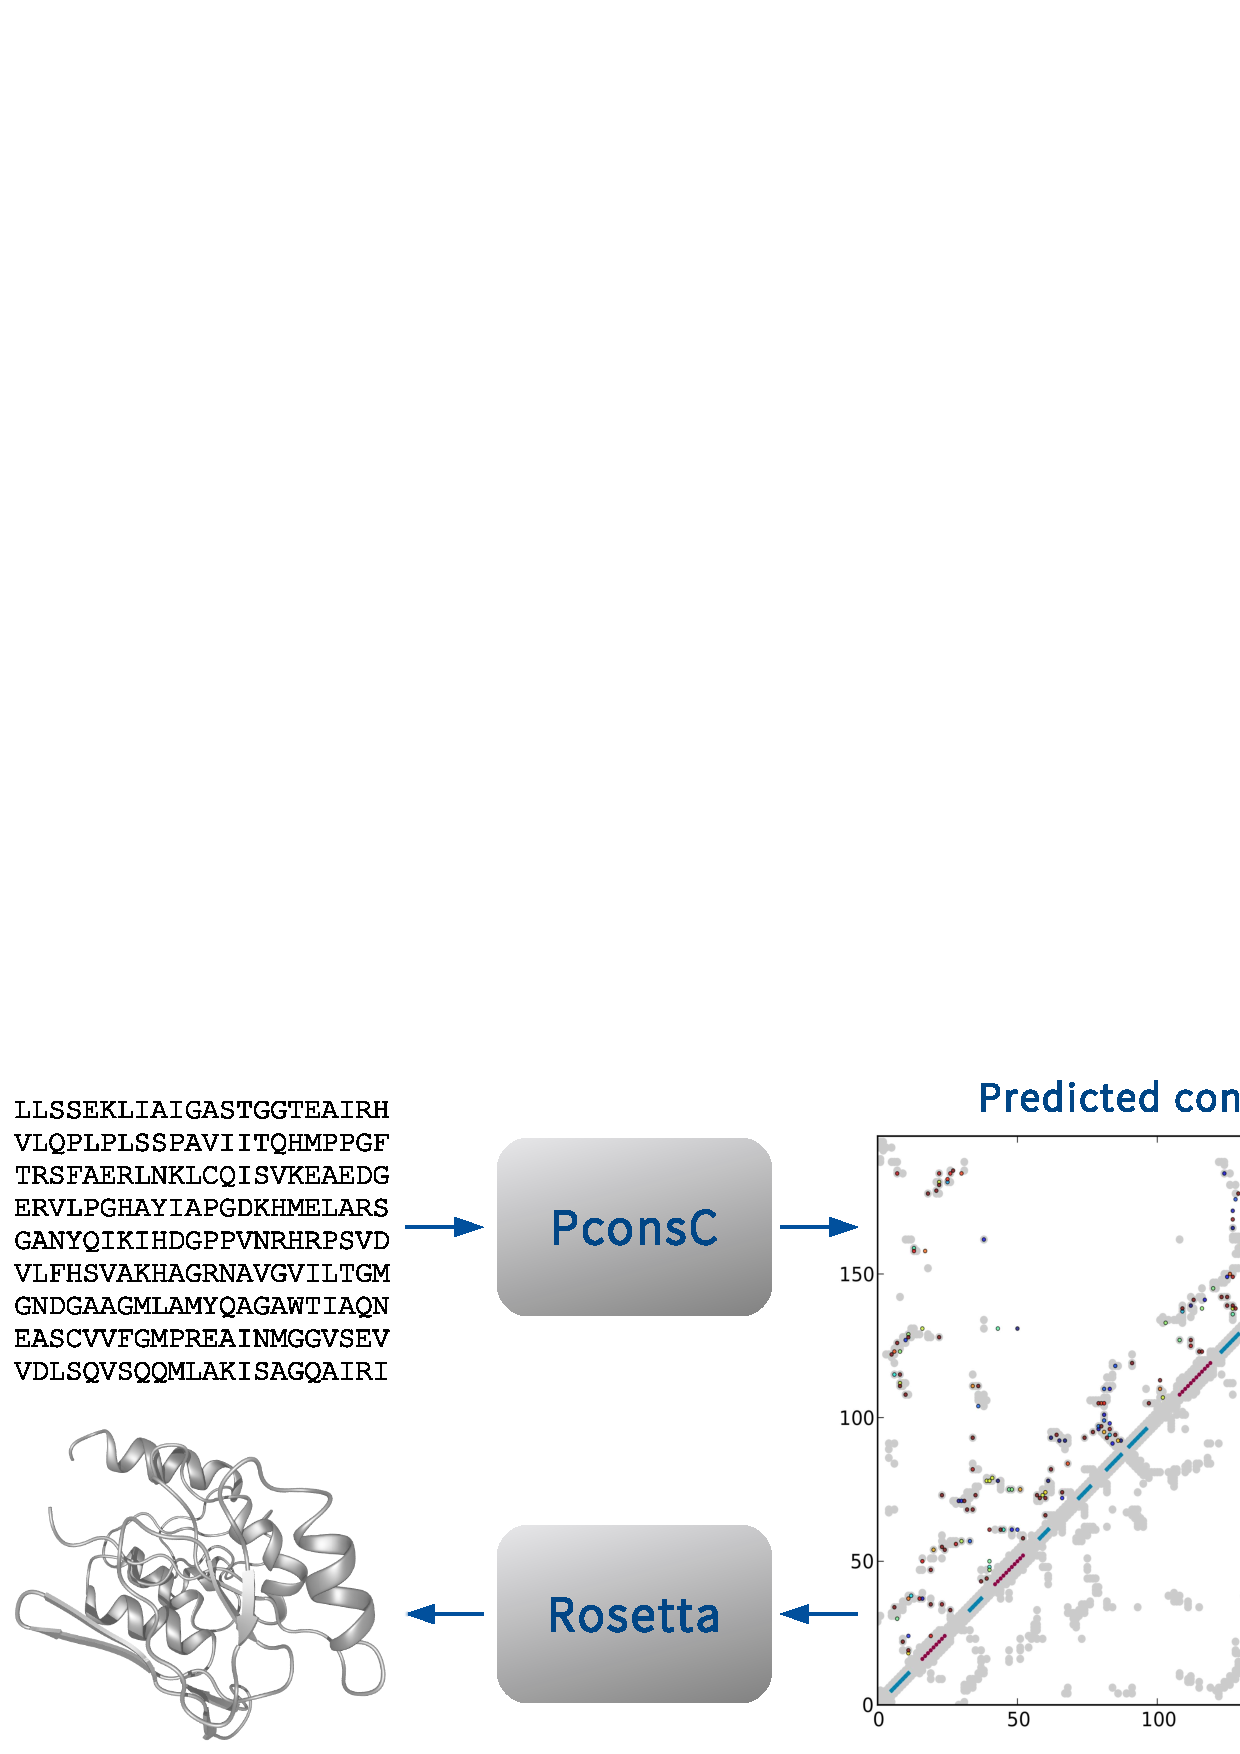
\includegraphics[scale=0.37]{figures/pipeline.png}}
\caption{PconsFold pipeline.}\label{fig:main}
\end{figure}
Rosetta: Fragment replacement by Markov chain Monte Carlo simulation / starting from extended amino acid chain / iteratively changing backbone dihedrals of parts of the chain according to selected fragment / calculate energy of the new conformation, then keep or dismiss it / works without residue contact information, but very slow convergence and only feasible for very small proteins / dramatic reduction in computational time when including contact information / therefore also applicable to larger proteins and more comprehensive studies possible (e.g. Pfam domain prediction) / \\


\end{methods}
\section{Algorithm}
\section{Implementation}
\section{Discussion}

\subsection{PconsFold}
For all results in this section, we used the internal Rosetta score to rank all predicted decoys. The top-ranked decoy structure was then selected as a final model. With the {\tt -nohoms} flag during fragment picking we ensured that all homologous structures are excluded. Only fragments from non-homologous protein structures were selected. This was done to simulate a real application case and not to overestimate model quality. If not stated otherwise, we used all 150 proteins of the PSICOV dataset as prediction targets in this section. \\\indent
Previous studies have shown that 20,000 -- 200,000 decoys are necessary to sample native-like conformations without using spatial constraints \cite[]{rosetta@home, rosetta_folding}. Figure \ref{fig:ros} (a) shows violin plots of the distributions of model quality, measured in TM-score. We reduced the number of decoy structures from 20,000 to 2,000. This corresponds to a 10-fold decrease of folding runtime but also leads to an expected decline in average model quality. The increased bulk at ~0.3 TM-score in the second distribution of Figure \ref{fig:ros} (a) represents an increased number of low quality models. We think the practical advantages of massively shorter Rosetta runs outweight slightly worse predicted models. This parameter is therefore set to a default value of 2,000 but can be specified by the user via a command line argument. All further results in this section are generated with this default setting. \\\indent
\begin{figure}[!tpb]%figure1
    \centerline{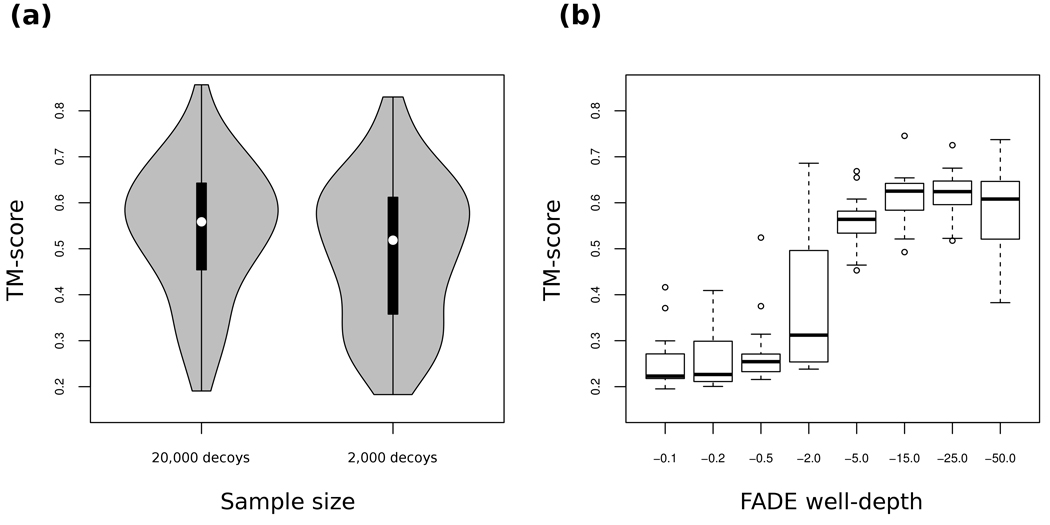
\includegraphics[scale=0.49]{figures/rosetta.jpg}}
\caption{Average TM-scores.}\label{fig:ros}
\end{figure}
We selected the FADE function to incorporate predicted residue contacts into Rosetta's native energy function. We then adjusted the parameter well-depth of FADE on a subset of 14 Proteins (Supplementary Table T2) of the PSICOV dataset. The resulting TM-scores are shown in Figure \ref{fig:ros} (b). The energy term from spatial constraints diminishes with well-depth values of -0.5 and above. This leads to a significant decrease in model quality. Lower values of -5.0 and below put a larger absolute weight on the constraints resulting in higher model qualities. We assume this is due to the small number of decoys we are generating in this experiment. We selected a value of -15.0 to achieve high model quality without outweighting Rosetta's native energy function completely.\\\indent
With any number of contacts used during structure prediction, the resulting model quality is on average higher than it would be without contact information. Figure \ref{fig:main} (a) shows average TM-scores for varying amounts of constraints. For each protein the number of top ranked contacts was selected relative to its sequence length. A value of 1.0 on the $x$-axis in Figure \ref{fig:main} (a) represents one contact per residue on average. The same Rosetta protocol as in PconsFold (green circles) was also applied to contacts from PSICOV (black squares) and plmDCA (blue triangles). Comparing $x=0.0$ to any other $x$ shows that predicted contacts generally improve model quality, regardless of method or amount of contacts. \\\indent
Improvements in contact prediction methods also increase the quality of predicted structures. With a maximal average TM-score of 0.55 PconsFold, i.e. using PconsC contacts, provides a 10\% improvement over using PSICOV or plmDCA contacts. This observation is consistent with a direct comparison of contact prediction methods as in \citeauthor{skwark_pconsc:_2013} \citeyear{skwark_pconsc:_2013}. However, the performance difference between PSICOV and plmDCA diminishes when their contacts are used in structure prediction. \\\indent
There is an optimal number of contacts, specific to the contact prediction method. In Figure \ref{fig:main} (a) the maximal average TM-score is reached at $x=1.0$ for PconsFold. For Rosetta/PSICOV and Rosetta/plmDCA a smaller number of one contact every other residue on average is optimal. This can also be explained by the quality of predicted contacts. A larger number of top ranked contacts is predicted with a higher quality in PconsC compared to plmDCA or PSICOV \cite[]{skwark_pconsc:_2013}. Using more of these contacts during structure prediction leads to improved models. \\\indent
This relation between contact and model quality can also be observed in Figure \ref{fig:main} (b). For each protein in the dataset the PPV of its contact map is plotted against the TM-score of the resulting model. The overall correlation between PPV and TM-score in this dataset is XX. \\\indent
Figure \ref{fig:main} (b) further indicates that $\alpha$-helical proteins (blue) are easier to fold than $\beta$-sheet containing proteins (green and yellow). Predicted contacts in $\alpha$-helical proteins can have lower PPV values, but resulting models remain as accurate, in terms of TM-score, as those of $\beta$-sheet containing proteins. 

\begin{figure}[!tpb]%figure1
    \centerline{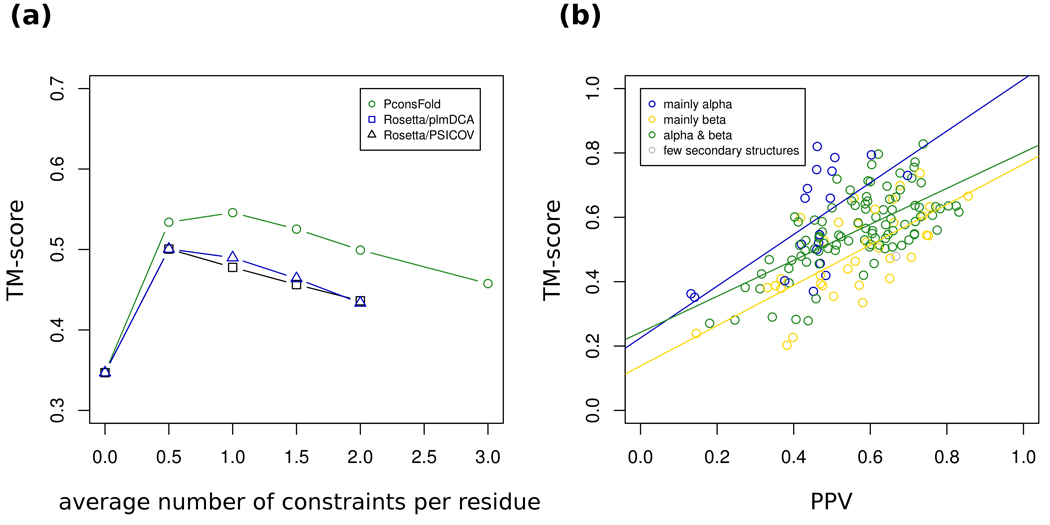
\includegraphics[scale=0.49]{figures/tmscores.jpg}}
\caption{(a) Average TM-scores. (b) TM-scores against PPV of underlying contact maps.}\label{fig:main}
\end{figure}

\subsection{Model quality assessment}

\begin{table}[!t]
\processtable{Average TM-scores for different QA tools\label{tab:qa}}
{\begin{tabular}{llll}\toprule
    Method  & EVfold & PconsFold & Rosetta/plmDCA \\ \midrule
    Rosetta & --     & 0.55     & 0.5          \\
    Pcons   & 0.47  & 0.53     & 0.47          \\
    Proq2   & 0.36  & 0.51     & 0.46          \\
    DOPE    & 0.46  & 0.36     & ~              \\ \botrule
\end{tabular}}{}
\end{table}

\subsection{Comparison to EVfold}

\begin{figure}[!tpb]%figure1
    \centerline{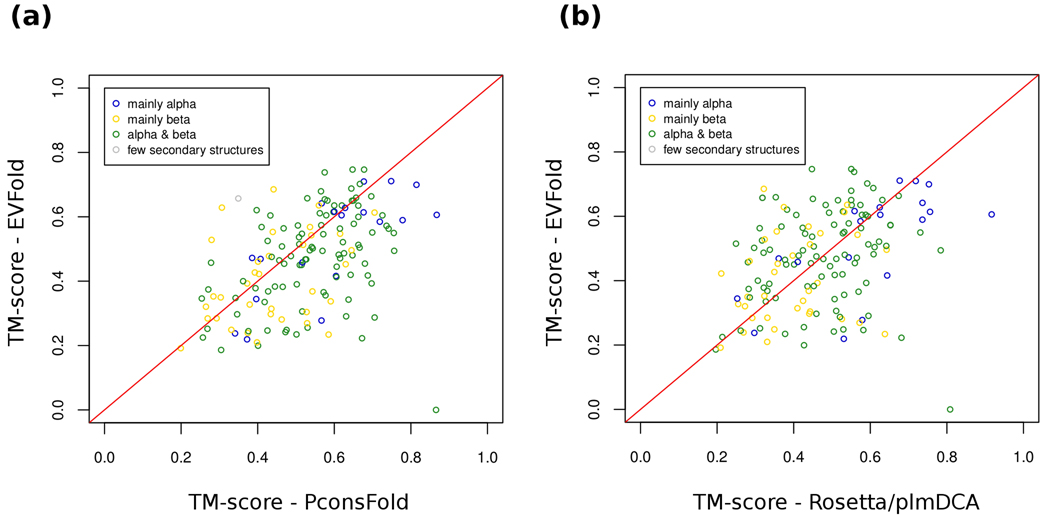
\includegraphics[scale=0.49]{figures/vs.jpg}}
\caption{PconsFold compared to EVfold.}\label{fig:vs}
\end{figure}

\begin{table}[!t]
\processtable{TM-scores for top ranked models. OLD (needs to be redone with selected QA)\label{tab:evfold}}
{\begin{tabular}{cccc}\toprule
    Protein      & EVfold (paper) & EVfold (web) & PconsFold \\ \midrule
    BPT1\_BOVIN  & 0.49   & 0.25           & 0.65      \\
    CADH1\_HUMAN & 0.55   & 0.54           & 0.54      \\
    CD209\_HUMAN & 0.39   & 0.64           & 0.54      \\
    CHEY\_ECOLI  & 0.65   & 0.66           & 0.83      \\
    ELAV4\_HUMAN & 0.57   & 0.61           & 0.5       \\
    O45418\_CAEEL & 0.48   & 0.62           & 0.28      \\
    OMPR\_ECOLI  & 0.35   & 0.44           & 0.48      \\
    OPSD\_BOVIN  & 0.5    & 0.55           & 0.55      \\
    PCB1\_HUMAN  & 0.25   & 0.43           & 0.43      \\
    RASH\_HUMAN  & 0.7    & 0.62           & 0.75      \\
    RNH\_ECOLI   & 0.54   & 0.66           & 0.62      \\
    SPTB2\_HUMAN & 0.37   & 0.51           & 0.6       \\
    THIO\_ALIAC  & 0.55   & 0.56           & 0.76      \\
    TRY2\_RAT    & 0.53*  & 0.78           & 0.83      \\
    YES\_HUMAN   & 0.35   & 0.31           & 0.55      \\ \midrule
    Mean         & 0.48   & 0.55           & 0.59      \\ \botrule
\end{tabular}}{}
\end{table}

\section{Conclusion}


\section*{Acknowledgement}
%Text Text Text Text Text Text  Text Text.  \citealp{Boffelli03} might want to know about  text text text text

\paragraph{Funding\textcolon} %Text Text Text Text Text Text  Text Text.

\bibliographystyle{natbib}
%\bibliographystyle{achemnat}
%\bibliographystyle{plainnat}
%\bibliographystyle{abbrv}
%\bibliographystyle{bioinformatics}
%
%\bibliographystyle{plain}
%
\bibliography{document}


%\begin{thebibliography}{}
%\bibitem[Bofelli {\it et~al}., 2000]{Boffelli03} Bofelli,F., Name2, Name3 (2003) Article title, {\it Journal Name}, {\bf 199}, 133-154.

%\bibitem[Bag {\it et~al}., 2001]{Bag01} Bag,M., Name2, Name3 (2001) Article title, {\it Journal Name}, {\bf 99}, 33-54.

%\bibitem[Yoo \textit{et~al}., 2003]{Yoo03}
%Yoo,M.S. \textit{et~al}. (2003) Oxidative stress regulated genes
%in nigral dopaminergic neurnol cell: correlation with the known
%pathology in Parkinson's disease. \textit{Brain Res. Mol. Brain
%Res.}, \textbf{110}(Suppl. 1), 76--84.

%\bibitem[Lehmann, 1986]{Leh86}
%Lehmann,E.L. (1986) Chapter title. \textit{Book Title}. Vol.~1, 2nd edn. Springer-Verlag, New York.

%\bibitem[Crenshaw and Jones, 2003]{Cre03}
%Crenshaw, B.,III, and Jones, W.B.,Jr (2003) The future of clinical
%cancer management: one tumor, one chip. \textit{Bioinformatics},
%doi:10.1093/bioinformatics/btn000.

%\bibitem[Auhtor \textit{et~al}. (2000)]{Aut00}
%Auhtor,A.B. \textit{et~al}. (2000) Chapter title. In Smith, A.C.
%(ed.), \textit{Book Title}, 2nd edn. Publisher, Location, Vol. 1, pp.
%???--???.

%\bibitem[Bardet, 1920]{Bar20}
%Bardet, G. (1920) Sur un syndrome d'obesite infantile avec
%polydactylie et retinite pigmentaire (contribution a l'etude des
%formes cliniques de l'obesite hypophysaire). PhD Thesis, name of
%institution, Paris, France.

%\end{thebibliography}
\end{document}
